\documentclass[UTF8]{ctexart}

\usepackage{ctex}
\CTEXsetup[format={\Large\bfseries}]{section}
\usepackage[top=28mm,bottom=28mm,left=15mm,right=15mm]{geometry}

\usepackage{fancyhdr}
\fancypagestyle{plain}{\pagestyle{fancy}}
\pagestyle{fancy}
\lhead{\kaishu 清华大学药学院药理毒理实验}
\newcommand{\numOfReport}[1]{\rhead{\kaishu 实验报告#1}}

\usepackage{fontspec}
\usepackage{wasysym}
\setCJKmainfont[AutoFakeBold={2}]{STZhongsong}
\setCJKmonofont{STZhongsong}

\usepackage{float}
\usepackage{booktabs}
\usepackage{tabularx}
\usepackage{array}
\usepackage{amsmath}
\usepackage{amsfonts}
\usepackage{amssymb}
\usepackage[figuresleft]{rotating}
\usepackage[para]{threeparttable}
\newcommand\info[2][40mm]{\underline{\makebox[#1][c]{#2}}}
\newcommand{\infoTable}[7]{
    \renewcommand\arraystretch{1.4}
    \begin{table}
        \begin{tabularx}{\textwidth}{
        >{\hsize=0.6\hsize\linewidth=\hsize}X
        >{\hsize=0.6\hsize\linewidth=\hsize}X
        >{\hsize=2.0\hsize\linewidth=\hsize}X
        >{\hsize=0.8\hsize\linewidth=\hsize}X
        }
            天气:\info[14mm]{#1} & 温度:\info[14mm]{#2 $^{\circ}\text{C}$} & 湿度:\info[14mm]{#3 $\%$} & 日期:#4\\
            姓名:\info[14mm]{#5} & 班级:\info[14mm]{#6} & 同组人:\info[70mm]{#7} & 
        \end{tabularx}
    \end{table}
}
\newcommand\columnC{\centering\arraybackslash}
\newcommand\columnL{\raggedright\arraybackslash}
\newcommand\columnR{\raggedleft\arraybackslash}

\usepackage{svg}
\usepackage{pdfpages}
\title{水合氯醛 $\text{ED}_{50} $ 的测定}
\author{}

\begin{document}
\infoTable{晴}{25}{60}{9/18/2024}{何昱晖}{药3}{荣子健、马逸然、赵方一澜}
\date{}
\maketitle

\section{实验目的和原理}

\subsection{实验目的}

掌握药物 $\text{ED}_{50}$ 和 $\text{LD}_{50}$ 的概念、原理、测定方法和意义,了解治疗指数的意义。

\subsection{实验原理}

\subsubsection{$\text{ED}_{50}$}

质反应量效曲线的横坐标为对数剂量,而纵坐标采用阳性反应发生的频数时,一般为正态分布曲线。如改用累加阳性频数为纵坐标时,可以得到标准的 S 型曲线。该曲线的中央部分($50\%$ 反应处)接近一条直线,斜率最大,其相应的剂量也就是能使群体中半数个体出现某一效应的剂量,通常称为半数效应量。如效应为疗效,则称半数有效量($\text{ED}_{50}$);如效应为死亡,则称半数致死量($\text{LD}_{50}$)。这些数值是评价药物作用强度和药物安全性的重要参数。\textbf{$\text{ED}_{50}$ 数值越小,药物的作用越强;$\text{LD}_{50}$ 越小,则药物的毒性越大}。

测定 $\text{ED}_{50}$ 和 $\text{LD}_{50}$ 的方法基本一致,只是所观察的指标不同,常用的测定方法有 Bliss 法(正规机率单位法),Litchfield-Wilcoxon 几率单位图解法,Kaerber 面积法,孙瑞元改进的 Kaerber 法(点斜法)及 Dixon-Mood 法(序贯法)等。其中序贯法需要的动物数最少,点斜法因其简捷性和精确性更为常用。

本次实验使用点斜法,应用点斜法时,实验设计须符合下面 3 点要求:

\begin{itemize}
    \item [(1)] 药物剂量设计为 $5\sim 8$ 组,应为等比数列,公比 $r=1.1\sim 1.6$;
    \item [(2)] 每剂量组动物数应一致,在 $10\sim 20$ 只范围内;
    \item [(3)] 各组动物的反应率大致符合正态分布。最大剂量($\text{D}_{\text{max}}$)组的阳性反应率应 $\geq 80\%$,最小剂量($\text{D}_{\text{min}}$)组的阳性反应率应 $\leq 20\%$。
\end{itemize}

若以 $\chi_m$ 为最大反应率组剂量的对数,$\mathrm{i}$ 为组间剂量比的对数(高剂量做分子),$p_k$ 为各组反应率,$\mathcal{P}_{\text{max}}$ 为最高反应率,$\mathcal{P}_{\text{min}}$ 为最低反应率,$n$ 为各组的动物数,则

$$
    \text{ED}_{50}=\lg^{-1}\left[\chi_m-\mathrm{i}\left(\sum_{k=1}^np_k-0.5\right)+\frac{\mathrm{i}}{4}(1-\mathcal{P}_{\text{max}}-\mathcal{P}_{\text{min}})\right]
$$

设 $\text{ED}_{50}$ 的 $95\%$ 可信限为 $t$,则

$$
    t=\lg^{-1}\left[\lg\text{ED}_{50}\pm 1.96\mathrm{i}\sqrt{\frac{\sum_{k=1}^n(p_k-p_k^2)}{n-1}}\right]
$$

\subsubsection{水合氯醛}

水合氯醛时一种有刺激性特臭的易挥发的麻醉用药物,对中枢神经系统有抑制作用,主要是抑制脑干网状结构上行激活系统,降低反射机能。\textbf{小剂量镇定,中等剂量催眠,大剂量产生全身麻醉和抗惊厥作用,超过浅麻醉剂量能抑制延髓呼吸中枢及血管运动中枢,导致死亡}。该药物消化道或者直肠给药能迅速吸收,脂溶性高,容易透过血脑屏障和胎盘,并可泌入乳液,1 小时达到峰值,持续 $4\sim 8$ 小时。水合氯醛由肝脏代谢,肾脏排泄。

\section{实验材料}

\begin{itemize}
    \item 实验仪器:天平、注射器(1ml)、鼠盒;
    \item 实验动物:ICR 小鼠(每组 10 只);
    \item 药品:水合氯醛溶液(212,251,296,349,412 mg/kg);
    \item 试剂:生理盐水。
\end{itemize}

\section{实验方法}

配制一系列水合氯醛溶液,剂量为 212,251,296,349,412 mg/kg。每只小鼠按照 0.1ml/10g 腹腔注射给药。

小鼠共分为 5 组,每组 2 只(全班共 6 个小组,每个给药剂量共计每组 12 只),腹腔基于不同剂量的水合氯醛溶液。

给药后观察 30min 内是否翻正反射小时,小鼠不翻正持续 1min 判定为阳性结果,将不同剂量组小鼠翻正反射消失的阳性数量填表。同时仔细观察小鼠在翻正反射消失前后的行为学变化,包括兴奋性的改变、1min 内小鼠理毛次数的多少。在给药 20min 后观察不同给药剂量组小鼠的行为学变化,其中安静不爱动为水合氯醛的镇静作用,闭目睡眠为催眠作用,翻正反射消失为中枢抑制的麻醉作用,更大剂量则出现呼吸抑制甚至死亡。

整合全班数据,计算各剂量的反应率和水合氯醛的 $\text{ED}_{50}$。

\pagebreak

\section{实验结果}

以下是我组的观察结果,表 1 是雄性小鼠的实验记录,表 2 是雌性小鼠的实验记录:

\begin{table}[H]
    \centering
    \begin{threeparttable}[b]
    \caption{本组中动物体重和性别及给药剂量}

    \quad
    
    \begin{tabularx}{\textwidth}{
        >{\columnC\hsize=0.3\hsize\linewidth=\hsize}X
        >{\columnC\hsize=0.4\hsize\linewidth=\hsize}X
        >{\columnC\hsize=0.3\hsize\linewidth=\hsize}X
        >{\columnC\hsize=0.4\hsize\linewidth=\hsize}X
        >{\columnC\hsize=0.3\hsize\linewidth=\hsize}X
        >{\columnC\hsize=4.3\hsize\linewidth=\hsize}X
    }
        \toprule[1.5pt]
        动物编号 & 体重\tnote{1} & 性别 & 给药剂量\tnote{2} & 给药量\tnote{3} & 动物行为学变化\\
        \midrule
        1 & 23 & \male & 212 & 0.23 & 少量出血(几滴),疑似注射至血管等非腹腔部位;小鼠 2min 后从兴奋变为安静少动,有蜷缩行为,呼吸正常;约 5min 时身体舒展,后脚脚心朝上,半闭目;9min 3s 时观察到翻正反射消失,且放回鼠笼后仍长时间睡眠。\\
        \midrule
        2 & 24 & \male & 251 & 0.24 & 注射后少许液体溢出,疑似注射至皮下;小鼠 5min 后从兴奋变为安静少动,呼吸正常;约 10min 时身体舒展,未闭目;在 5、10、15、20、25、30 min 所进行的检查中均未发生翻正反射消失的现象。\\
        \midrule
        3 & 23 & \male & 296 & 0.23 & 注射后小鼠有舔舐腹部行为;2min 内小鼠爬行步态变得蹒跚;约 5min 时身体舒展,后脚脚心朝上,闭目;在 5min 时第一次检查,出现抽搐但具有翻正反射;10min 40s 时观察到翻正反射消失,且放回鼠笼后仍长时间睡眠。\\
        \midrule
        4 & 22 & \male & 349 & 0.22 & 注射后小鼠迅速由躁动变为安静,有蜷缩现象;约 3min 时出现一次突然抽搐;约 5min 时身体舒展且闭目睡眠;5min 时观察到翻正反射消失,且放回鼠笼后仍长时间睡眠。\\
        \midrule
        5 & 21 & \male & 412 & 0.21 & 注射后小鼠在 2min 内由躁动变为安静,间断爬行但爬行步态逐渐蹒跚;5min 时身体舒展,后脚脚心朝上,闭目;在 5min时第一次检查,出现抽搐但具有翻正反射(疑似借鼠盒壁支撑力翻身);11min 时观察到翻正反射消失,且放回鼠笼后仍长时间睡眠。\\
        \bottomrule[1.5pt]
    \end{tabularx}
    \begin{tablenotes}
        \item[1] 单位 g
        \item[2] 单位 mg/kg
        \item[3] 单位 ml
    \end{tablenotes}
    \end{threeparttable}
\end{table}

\begin{table}[H]
    \centering
    \begin{threeparttable}[b]
    \caption{本组中动物体重和性别及给药剂量(续表)}

    \quad
    
    \begin{tabularx}{\textwidth}{
        >{\columnC\hsize=0.3\hsize\linewidth=\hsize}X
        >{\columnC\hsize=0.4\hsize\linewidth=\hsize}X
        >{\columnC\hsize=0.3\hsize\linewidth=\hsize}X
        >{\columnC\hsize=0.4\hsize\linewidth=\hsize}X
        >{\columnC\hsize=0.3\hsize\linewidth=\hsize}X
        >{\columnC\hsize=4.3\hsize\linewidth=\hsize}X
    }
        \toprule[1.5pt]
        动物编号 & 体重\tnote{4} & 性别 & 给药剂量\tnote{5} & 给药量\tnote{6} & 动物行为学变化\\
        \midrule
        6 & 22 & \female & 212 & 0.22 & 小鼠注射后频繁运动,2min 时变为安静少动,可见明显呼吸,难以人为翻动;约 12min 时达成翻正反射消失,呈侧躺状睡眠;约 40min 时苏醒并再度活跃爬动。\\
        \midrule
        7 & 23 & \female & 251 & 0.23 & 小鼠注射后频繁运动,但平衡性不佳,直立能力变差;1min 时变为安静少动;约7min时达成翻正反射消失,呈侧躺状睡眠,伴有少许抽搐;约50min时苏醒并再度活跃爬动。\\
        \midrule
        8 & 20 & \female & 296 & 0.20 & 小鼠注射后约1min时变为安静少动,有少量理毛行为;约5min时达成翻正反射消失,呈侧躺偏仰躺状睡眠,四肢呈僵直状。\\
        \midrule
        9 & 23 & \female & 349 & 0.23 & 小鼠注射后有迟缓爬动,迅速变为安静少动;约4min时达成翻正反射消失,进入睡眠。\\
        \midrule
        10 & 22 & \female & 412 & 0.22 & 小鼠注射后有激烈爬动,方向感与攀援能力变差;约3min时达成翻正反射消失,进入睡眠。\\
        \bottomrule[1.5pt]
    \end{tabularx}
    \begin{tablenotes}
        \item[4] 单位 g
        \item[5] 单位 mg/kg
        \item[6] 单位 ml
    \end{tablenotes}
    \end{threeparttable}
\end{table}

\begin{table}[H]
    \centering
    \caption{小鼠腹腔注射不同剂量水合氯醛溶液后 30min 内翻正反射消失情况——全班数据汇总}
    
    \quad

    \begin{tabularx}{\textwidth}{
        >{\columnC\hsize=1\hsize\linewidth=\hsize}X
        >{\columnC\hsize=1\hsize\linewidth=\hsize}X
        >{\columnC\hsize=1\hsize\linewidth=\hsize}X
        >{\columnC\hsize=1\hsize\linewidth=\hsize}X
        >{\columnC\hsize=1\hsize\linewidth=\hsize}X
    }
        \toprule[1.5pt]
        组别 & 剂量(mg/kg) & 每组只数 & 阳性反应动物数 & 阳性反应率\\
        \midrule
        1 & 212 & 12 & 6 & $50.00\%$\\
        \midrule
        2 & 251 & 12 & 5 & $41.67\%$\\
        \midrule
        3 & 296 & 12 & 12 & $100.00\%$\\
        \midrule
        4 & 349 & 12 & 12 & $100.00\%$\\
        \midrule
        5 & 412 & 12 & 11 & $91.67\%$\\
        \bottomrule[1.5pt]
    \end{tabularx}
\end{table}

$$
    \text{ED}_{50}=\lg^{-1}\left(\lg 412-\lg 1.18\times\left(\frac{23}{6}-0.5\right)\right)=237.296 \text{ml}\cdot\text{kg}^{-1}
$$

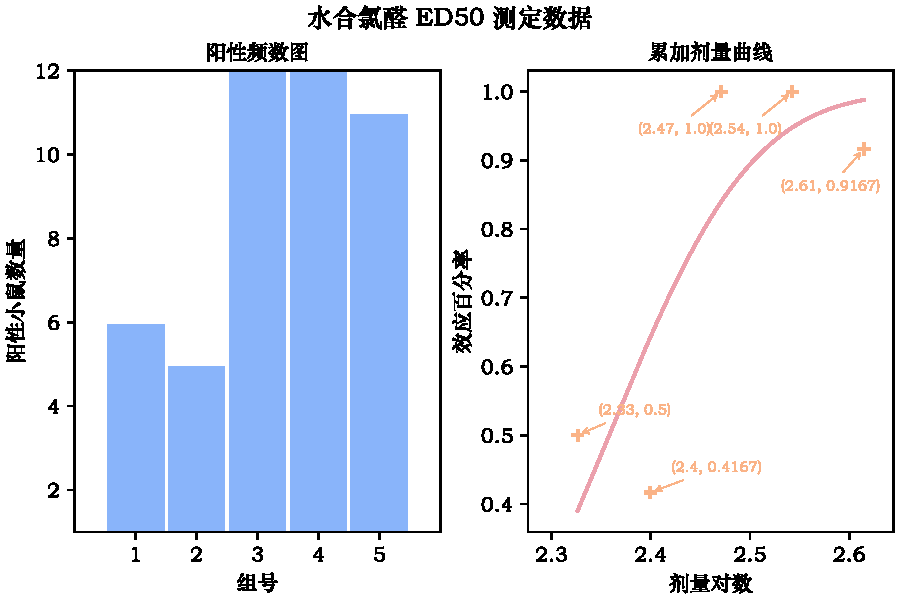
\includepdf[page=1]{figure-1_svg.pdf}
\end{document}